\chapter{Implementação do algoritmo}
\label{chap:implementacao}
Neste capítulo são apresentadas as ferramentas e técnicas utilizadas para a implementação do algoritmo, testes de performance realizados, dificuldades encontradas e a evolução da implementação durante seu processo de desenvolvimento.

\section{Clojure}
Clojure é uma linguagem de propósitos gerais, dinâmica e funcional, lançada em 2007, por Rich Hickey.
Por se tratar de um dialeto de Lisp\footnote{Lisp (LISt Processing) teve sua primeira especificação em 1958 e foi originalmente pensada como uma notação matemática prática para programas de computador, influenciada pelo Cálculo-$\lambda$ de Alonzo Church. A linguagem ainda é uma das linguagens mais antigas ainda utilizadas largamente no momento da escrita deste texto.}, Clojure foi criada com o intuito de preservar o caráter funcional e poderoso de Lisp para resolver problemas atuais como concorrência e paralelismo numa roupagem mais moderna.

Como se trata de uma implementação do paradigma funcional, a computação dos dados é encarada como avaliações de funções matemáticas, que favorecem o fraco acoplamento entre módulos e incentiva o uso de recursões evitando efeitos colaterais, uma vez que dados são considerados imutáveis nessa linguagem.

Para este trabalho foi utilizada a última implementação estável\footnote{Foi utilizada a versão 1.2, disponível em http://clojure.org/downloads. Último acesso em 20 de novembro de 2010.} da linguagem Clojure no momento da escrita deste texto.


\section{Desenvolvimento}
Preocupações como performance e corretude permearam o processo e técnicas de desenvolvimento ágil como TDD (Test Driven Development)\footnote{Test Driven Development consiste em um processo de desenvolvimento de software em que testes são escritos antes do desenvolvimento do código em si, facilitando o entendimento e condução do processo de raciocínio sobre o problema, além de contribuir como documentação do código.} foram utilizadas durante sua execução.

Todas as funções criadas acompanham testes unitários. Tais testes não garantem totalmente que o código é  correto, mas oferecem um meio de assegurar que alguns casos previamente pensados em que o algoritmo poderia falhar estão cobertos e uma garantia maior pode ser dada para futuros usuários e mantenedores do código.

Nenhuma particularidade do sistema em que foi incorporado este algoritmo -- descrito no capítulo \ref{chap:holmes} -- foi incluída na implementação. Deste modo, o mesmo código pode ser encarado como uma caixa preta e pode ser incorporado em outro sistema com facilidade. Como a linguagem Clojure é compilada para a JVM (Java Virtual Machine), o código também pode ser executado na maioria dos sistemas operacionais existentes atualmente.

\section{Performance}
Apesar do algoritmo apresentado no capítulo \ref{chap:pip} não representar muitas dificuldades de entendimento, implementá-lo de uma forma eficiente requereu pesquisa sobre as estruturas de dados adequadas e detalhes da linguagem para a realização da tarefa.

A implementação do código passou por diversas modificações para atender aos requisitos de performance exigidos pelo projeto. Foram desenvolvidas três versões -- incluídas no Apêndice -- e suas evoluções serão brevemente descritas na próxima seção.

\subsection{Otimizações}
\subsubsection{Versão 1}
A primeira versão do algoritmo -- anexo \ref{chap:versao1} -- foi desenvolvida sem grandes otimizações. Não foi utilizado nenhum mecanismo de cache de resultados intermediários, nem testes muito robustos.

Nesta versão foram definidas as estruturas de dados a serem utilizadas. Para a lista de entrada, se preferiu utilizar \textit{vectors}, que possuem complexidade $O(1)$ para acesso aleatório. Durante o processamento, mantém-se um \textit{vector} que cresce a cada iteração, com os índices na série original para os PIPS escolhidos. Como durante o processamento, são armazenados apenas os índices -- ao invés da combinação $(x, y)$ de cada ponto -- ao se calcular as distâncias são necessários acessos aleatórios a série original para se buscar os pontos. A cada iteração, o \textit{vector} de PIPs é ordenado.

Como os tempos de execução apresentados ficaram bem aquém do desejado, a implantação em um software real -- um dos objetivos pretendidos com esse trabalho, apresentados na seção \ref{sec:objetivos} -- se tornou impeditiva.  Foi necessário, portanto, o desenvolvimento de uma versão de melhor desempenho.


\subsubsection{Versão 2}
Para a segunda versão foram implementadas algumas melhorias. A mais importante de todas se deveu a percepção de que cálculos de distância eram repetidos desnecessariamente. Foi buscada, deste modo, uma solução de cacheamento dos resultados e para tanto, utilizou-se a função \textit{memoize} da linguagem Clojure, que contribuiu para a melhora significativa no tempo de execução.

A cada iteração são armazenados os intervalos entre pips em um \textit{hashset}. A vantagem de se armazenar os intervalos é que os mesmos podem ser avaliados em paralelo -- dependendo de uma sincronização no término para se analisar a melhor distância -- apesar de não ter se utilizado nenhuma espécie de paralelismo nessa versão. Com essa alteração, a necessidade de se ordenar a lista de PIPs a cada iteração passou a inexistir. 

A escolha de um \textit{hashset} se deve a dois motivos. O primeiro deles é que se pode garantir que se a entrada possuir pontos duplicados, estes não aparecerão na saída do algoritmo. O segundo motivo é que como os intervalos são divididos a cada iteração, precisamos redefinir a lista de intervalos, retirando o intervalo anterior, criando dois novos intervalos, no ponto em que o novo PIP foi encontrado. Acessos aleatórios em \textit{hashsets} ocorrem em tempo $O(log_{32}n)$, que na prática pode ser considerado constante.


Como são processadas listas muito extensas e sua avaliação pode ser custosa, optou-se também nesta versão por se utilizar \textit{lazy sequences}\footnote{Para maiores detalhes sobre o conceito de \textit{lazy sequences}, veja~\cite{programmingclojure}}. Como muitos programas escritos em Clojure envolvem computação de listas, a linguagem fornece esse mecanismo para se construir expressões complexas e extensas que só são avaliadas quando realmente são necessárias. Listas infinitas podem ser definidas com esse recurso.

Outra melhoria surgida nessa versão se deu ainda com relação ao cálculo de distâncias. Como são efeituados muitos cálculos de distâncias, foi buscada nessa versão uma implementação mais eficiente. Para isso, substituiu-se o uso da função \textit{abs} do pacote \verb+clojure.contrib.generic.math-functions+ pela versão mais performática da função \textit{abs}, do pacote \verb+clojure.contrib.math+.

Como Clojure é uma linguagem construída por cima da linguagem Java, casting para tipos primitivos para esta linguagem -- discutido em~\cite{practicalclojure}, onde podem ser encontrados outras técnicas para se aumentar o desempenho de programas em Clojure -- também foram adicionados.


\subsubsection{Versão 3}
A versão 3, última desenvolvida, é a que oferece o menor tempo de execução dentre todas as anteriores.
Ao invés de definirmos nossas \textit{lazy sequences}, foi preferida a utilização da função \textit{iterate}, disponível no \textit{core} da linguagem. A função \textit{iterate} recebe como parâmetro uma função e um parâmetro adicional. No momento de sua chamada, a função passada como argumento é executada com o argumento adicional e a sua saída é aplicada a mesma função. O comportamento pode ser continuado indefinidamente. Isso evita muitas trocas de contexto e avaliações de listas muito extensas previamente.

Fez-se uso de mais \textit{lazy sequences} onde necessário e ganhos de performance consideráveis foram conseguidos quando casting para tipos primitivos foram acrescentados no código.

\subsubsection{Testes de performance}
Para comparar a evolução das implementações foram executadas as três versões em ambiente controlado para séries aleatórias e comparados seus tempos de execução.

A máquina utilizada possui as seguintes configurações:
\begin{itemize}
\item Processador: Intel Celeron processor 560, 2.13 GHz, 1 MiB L2 cache
\item Memória Principal: 1 GiB
\item Sistema Operacional: Ubuntu Linux versão 10.04
\end{itemize}

Na tabela \ref{tab:tempos-100} é possível ver um resumo dos tempos de execução para testes realizados com séries aleatórias -- para não privilegiar nenhuma das versões -- de 100 pontos e 1000 pontos. Foram executadas 500 rodadas para cada valor de PIPs e tirada sua média para atender a Lei dos Grandes Números e garantir uma baixa variância nos resultados. Pode-se observar que a Versão 1 destoa bastante das outras duas versões.

\begin{table}[htb!]
  \begin{center}
      \begin{tabular}{ | c | c | c | c | }
      \hline
      \multicolumn{4}{|c|}{Tempos de execução} \\
      \hline
      Número de PIPs & Versão 1 & Versão 2 & Versão 3 \\ \hline
      4 & 7.49943    & 1.8605996 & 0.6156479 \\ \hline
      10 & 26.238653 & 2.321418  & 1.0887681 \\ \hline
      20 & 54.226994 & 4.5783596 & 1.3933954 \\ \hline
      30 & 84.99333  & 5.6005797 & 2.06694   \\ \hline
      40 & 115.92436 & 7.35721   & 3.0876982 \\ \hline
      50 & 145.32526 & 9.438611  & 3.6283286 \\ \hline
      60 & 156.99683 & 12.641098 & 4.9837728 \\ \hline
      70 & 171.61131 & 14.659222 & 5.6078625 \\ \hline
      80 & 174.81184 & 15.915979 & 7.315132  \\ \hline
      90 & 189.28699 & 18.447191 & 8.141004  \\
      \hline
      \end{tabular}
  \end{center}
  \caption[Tempos de execução]{Tempos de execução para as três versões implementadas do algoritmo PIP para séries com 100 pontos. Os tempos estão em milissegundos.}
  \label{tab:tempos-100}
\end{table}


\begin{table}[htb!]
  \begin{center}
      \begin{tabular}{ | c | c | c | c | }
      \hline
      \multicolumn{3}{|c|}{Tempos de execução} \\
      \hline
      Número de PIPs & Versão 2 & Versão 3 \\ \hline
      100 & 239.5926  & 101.20084 \\ \hline
      200 & 342.2604  & 184.52263 \\ \hline
      300 & 396.32697 & 163.0423  \\ \hline
      400 & 538.5814  & 217.53302 \\ \hline
      500 & 706.6794  & 328.58374 \\ \hline
      600 & 952.6192  & 394.18314 \\ \hline
      700 & 1071.5186 & 481.18253 \\ \hline
      800 & 1279.3595 & 561.9523  \\ \hline
      900 & 1397.1849 & 708.9733  \\
      \hline
     \end{tabular}
  \end{center}
  \caption[Tempos de execução para as duas melhores versões]{Tempos de execução para as duas melhores versões implementadas do algoritmo PIP para séries com 1000 pontos. Os tempos estão em milissegundos.}
  \label{tab:tempos-1000}
\end{table}

É possível observar também que a Versão 3 é duas vezes mais rápida que a Versão 2 analisando os valores da tabela \ref{tab:tempos-1000}. Um ganho considerável de performance quando séries com alta dimensionalidade  devem ser processadas. Nas figuras \ref{fig:comp-3-versions} e \ref{fig:comp-2-versions}, podem ser vistos os mesmos dados de forma gráfica.

\begin{figure}[htb!]
  \begin{center}
    \subfloat[Comparação entre os tempos de execução das três versões implementadas. Série original possuía 100 pontos.]{\label{fig:comp-3-versions}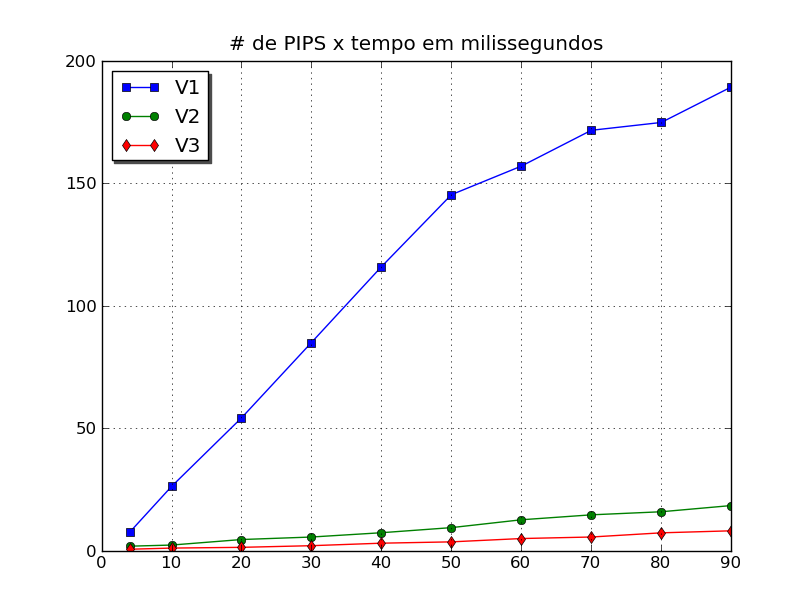
\includegraphics[width=0.5\textwidth]{execution-time-3-versions-100-points}}
    \\
    \subfloat[Comparação entre os tempos de execução das duas melhores versões implementadas. Série original possuía 1000 pontos.]{\label{fig:comp-2-versions}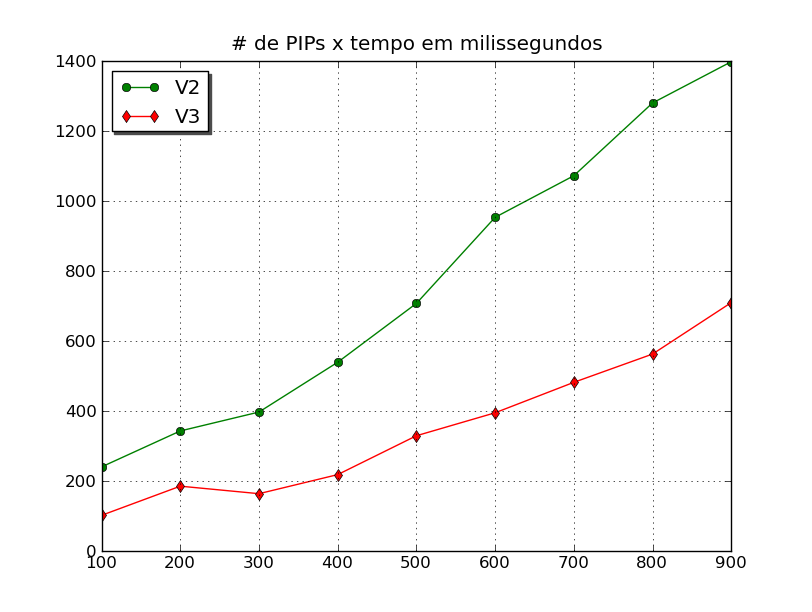
\includegraphics[width=0.5\textwidth]{execution-time-2-versions-1000-points}}
    \centering
    \caption[Comparativo entre as 3 versões implementadas]{Tempos de execução para as implementações do algoritmo PIP}
    \label{fig:comparativo}
  \end{center}
\end{figure}
